% 1. Стиль и язык
\documentclass[14pt]{report} % Стиль (по умолчанию будет 14pt)

% Остальные стандартные настройки убраны в preamble.inc.tex.
%\include{preamble.inc}
\usepackage[russian]{babel}
%\usepackage{dashrule}
\usepackage{graphicx}
\usepackage{geometry}
\usepackage{wrapfig}
\usepackage{listings}
\usepackage{setspace}
\usepackage{indentfirst}
\linespread{1.3}
\usepackage[14pt]{extsizes}
\geometry{top=2cm}
\geometry{bottom=2cm}
\geometry{right=1cm}
\geometry{left=2cm}

\usepackage{float}



\usepackage{amsmath,amsfonts,amssymb,amsthm} 

\lstset{ %
language=c++,                 % выбор языка для подсветки (здесь это С++)
basicstyle=\small\sffamily, % размер и начертание шрифта для подсветки кода
numbers=left,               % где поставить нумерацию строк (слева\справа)
numberstyle=\tiny,           % размер шрифта для номеров строк
stepnumber=1,                   % размер шага между двумя номерами строк
numbersep=5pt,                % как далеко отстоят номера строк от подсвечиваемого кода
showspaces=false,            % показывать или нет пробелы специальными отступами
showstringspaces=false,      % показывать или нет пробелы в строках
showtabs=false,             % показывать или нет табуляцию в строках
frame=single,              % рисовать рамку вокруг кода
tabsize=2,                 % размер табуляции по умолчанию равен 2 пробелам
captionpos=t,              % позиция заголовка вверху [t] или внизу [b] 
breaklines=true,           % автоматически переносить строки (да\нет)
breakatwhitespace=false, % переносить строки только если есть пробел
escapeinside={\#*}{*)}   % если нужно добавить комментарии в коде
}

% Для измененных титулов глав:
\usepackage{titlesec, blindtext, color} % подключаем нужные пакеты
\definecolor{gray75}{gray}{0.75} % определяем цвет
\newcommand{\hsp}{\hspace{20pt}} % длина линии в 20pt
% titleformat определяет стиль
%\titleformat{\chapter}[hang]{\Huge\bfseries}{\thechapter\hsp\textcolor{gray75}{|}\hsp}{0pt}{\Huge\bfseries}
\titleformat{\chapter}%
  {\normalfont\bfseries\Huge}{\thechapter.}{10pt}{}
\titlespacing*{\chapter}{0pt}{20pt}{20pt}
%\newpagestyle{mystyle}{
%  \sethead[][\thechapter.\enspace\chaptertitle][]{}{\thesection~\sectiontitle}{}
%\setfoot{}{\thepage}{}}
% Настройки листингов.
\DeclareGraphicsExtensions{.pdf,.png,.jpg, .svg}
\graphicspath{{./graphics/}}
%\appendix   % Тут идут приложения

%\addto\captionsrussian{\def\thebibliography{Список литературы}}
%\bibliographystyle{gost780u}
%\bibliography{bibliography}

%\usepackage{caption} %заголовки плавающих объектов
%\captionsetup[table]{justification=centering} %установки для заголовков таблиц
\usepackage{caption} \captionsetup[table]{labelsep=endash,justification=justified,singlelinecheck=false,font=normalsize} 

\setcounter{tocdepth}{1}
%\DeclareUnicodeCharacter{00A0}{ }


\begin{document}
\def\contentsname{Содержание}



\begin{titlepage}
    


    \noindent \begin{minipage}{0.20\textwidth}
        
\includegraphics[width=3.7cm]{BMSTU.svg}
    \end{minipage}
    \noindent\begin{minipage}{0.8\textwidth}\centering \singlespacing\small
        \textbf{Министерство науки и высшего образования Российской Федерации}\\
        \textbf{Федеральное государственное бюджетное образовательное учреждение высшего образования}\\
        \textbf{«Московский государственный технический университет \\ имени Н.Э.~Баумана}\\
        \textbf{(национальный исследовательский университет)»}\\
        \textbf{(МГТУ им. Н.Э.~Баумана)}
    \end{minipage}
    
    \noindent\rule{18cm}{3pt}


    \begin{flushleft}
    \small{ФАКУЛЬТЕТ \underline{«Информатика и системы управления»}\\    
    КАФЕДРА \underline{«Программное обеспечение ЭВМ и информационные технологии»}}\\
    ДИСЦИПЛИНА \underline{«Анализ алгоритмов»}
    \end{flushleft}

    \
    
    \ 
    
    \ 
    
    \ 
    %\newline\newline\newline\newline\newline\newline\newline
    
    \begin{center}
        \Large\textbf{Лабораторная работа № 6}
    \end{center}


    \begin{flushleft}
        \textbf{Дисциплина} \underline{Анализ алгоритмов}\\
        \textbf{Тема} \underline{Муравьиный алгоритм}\\
        \textbf{Студент} \underline{Боренко А. Д.}\\
        \textbf{Группа} \underline{ИУ7-52Б}\\
        \textbf{Оценка (баллы)} \underline{~~~~~~~~~~~~~~~}\\
        \textbf{Преподаватель} \underline{Волкова Л.Л.}
    \end{flushleft}
    
        
    \begin{center}
        \vfill
        Москва --- \the\year г.
    \end{center}

\end{titlepage}

\setcounter{page}{2} 

\tableofcontents 

\chapter*{Введение}\label{Input}
\addcontentsline{toc}{chapter}{Введение}



Параллельные вычисления — способ организации компьютерных вычислений, при котором программы разрабатываются как набор 
взаимодействующих вычислительных процессов, работающих параллельно (одновременно). 

Причины для использования параллелизма:

\begin{enumerate}
  \item разделение обязанностей;
  \item повышение производительности.
\end{enumerate}

Разделение обязанностей почти всегда приветствуется при разработке программ: если сгруппировать взаимосвязанные и разделить 
несвязанные части кода, то программа станет проще для понимания и тестирования и, стало быть, будет содержать меньше ошибок. 

Повысить производительность можно 2 способами: разбить задачу на части и запустить их
параллельно, уменьшив тем самым общее время выполнения и воспользоваться имеющимся параллелизмом для решения
более крупных задач, например, обрабатывать не один файл за раз, а сразу два, десять или двадцать, - способы 
называются распараллеливание по задачам и по данным, соответственно.

Целью данной работы является разработка и исследования параллельных алгоритмов нахождения среднего арифметического матрицы.
Задачами данной лабораторной являются:
\begin{enumerate}
  %\item изучение алгоритмов сортировки пузырьком, вставками, выбором;
  \item реализация последовательного алгоритма нахождения среднего арифметического матрицы;
  \item реализация распараллеленного алгоритма нахождения среднего арифметического матрицы;
  \item сравнительный анализ реализованных алгоритмов;
  \item описание и обоснование полученных результатов в отчете о выполненной лабораторной работе, выполненного как расчетно-пояснительная 
        записка к работе.
\end{enumerate}

\chapter{Аналитическая часть}\label{Analis}
%\addcontentsline{toc}{chapter}{1 Аналитическая часть}

В данном разделе будут рассмотрен алгоритм нахождения среднего арифметического матрицы и
идея его параллельной реализации.

\section{Последовательный алгоритм нахождения среднего арифметического матрицы}\label{BubbleSort}

Последовательно суммируются все элементы матрицы, а после делятся на их количество - строки * столбцы.

\section{Распараллеленный алгоритм нахождения среднего арифметического матрицы}\label{ChoiseSort}

Для увеличения производительности приведенный алгоритм можно распараллелить. Рассмотрим два способа распараллеливания: по строкам и
столбца. В первом случае каждый поток обрабатывает элементы своих строк (эти строки обрабатываются только им). Во втором каждый поток 
обрабатывает элементы своих столбцов.

На рисунке \ref{ris:ill} показан принцип распараллеливания по строкам.

\begin{figure}[H]
  \center{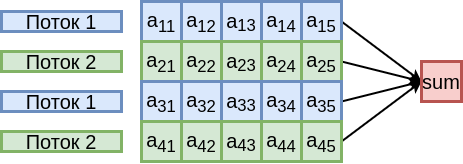
\includegraphics[scale=0.7]{l1.il}}
  \caption{Принцип работы распараллеленого алгоритма}
  \label{ris:ill}
\end{figure}


\section{Вывод аналитической части}\label{End_analis_chapter}

В данной работе стоит задача реализации следующих алгоритмов: последовательного алгоритма нахождения среднего арифметического матрицы,
распараллеленого по строкам алгоритма нахождения среднего арифметического матрицы, распараллеленого по столбцам алгоритма нахождения
среднего арифметического матрицы. Необходимо сравнить алгоритмы умножения матриц по эффективности по времени.
 


\chapter{Конструкторская часть}\label{Konstruct}
%\addcontentsline{toc}{chapter}{2 Конструкторская часть}

В данном разделе представлены схемы алгоритмов. Так же будут описаны пользовательские структуры данных, 
приведены классы эквивалентности для тестирования реализуемого ПО.

\section{Схема алгоритмов}\label{SchemaAlg}

На рисунке \ref{ris:schemaposav} показана схема алгоритмов работы диспетчера и каменщиков.

\begin{figure}[H]
  \center{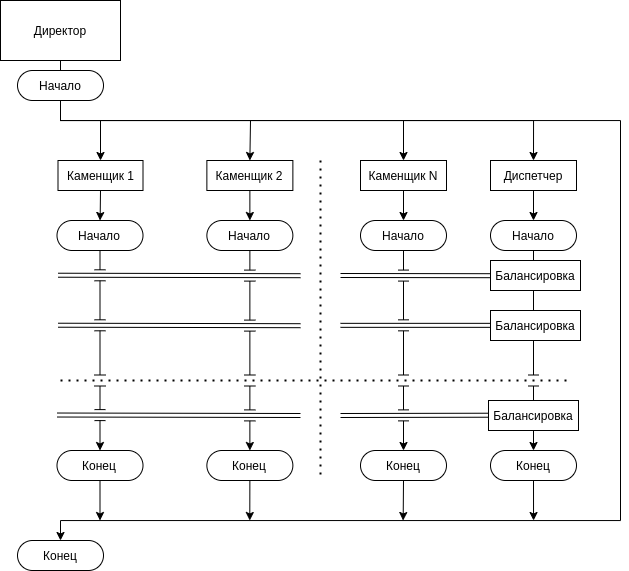
\includegraphics[scale=0.40]{l1.res}}
  \caption{Схема алгоритма полного перебора}
  \label{ris:schemaposav}
\end{figure}

\section{Структуры данных}\label{Structs}

При реализации приведенных алгоритмов потребуются типы данных: матрица кирпичей, кирпич, параметры системы.

Кирпич:

\begin{enumerate}
  \item название строителя 
  \item значение bool - установлен, или нет
\end{enumerate}

Параметры:

\begin{enumerate}
  \item ширина стены;
  \item высота стены;
  \item стартовая очередь кирпичей; 
  \item количество каменщиков;
  \item границы участков каждого каменщика;
  \item массив значений, где i - ое значение - количество установленных каменщиком.
\end{enumerate}
%\subsection{Способы тестирования}\label{TestingMethods}

%При разработке программы удобно использовать следующие методы тестирования:

%\begin{enumerate}
%    \item Модульные тесты 
%    \item Функциональные тесты 
%\end{enumerate}

\section{Вывод конструкторской части}\label{KonstructResult}

На основе данных, полученных в аналитическом разделе, была построена схема используемого алгоритма,
выделены необходимые для реализации структуры данных.



\chapter{Технологическая часть}\label{tecnology}
%\addcontentsline{toc}{chapter}{3 Технологическая часть}

\section{Требования к ПО}\label{Requirements}

Требования к программному обеспечению:
\begin{enumerate}
    \item на вход подается количество заявок;
    \item результат: замеры времени пребывания заявки на этапах и в очередях. 
\end{enumerate}

\section{Выбор языка программирования}\label{Language}

Был выбран язык go, поскольку он удовлетворяет необходимым требованиям и удобен программирования параллельных вычислений. 
Средой разработки выбрана Visual Studio Code.

\section{Структуры данных}\label{StructsList}

На листинге \ref{list:matrixstruct} представлено описание структуры заявки.

\begin{lstinputlisting}
    [caption = {Структура матрицы},
    label = {list:matrixstruct},
    linerange={30-39},
    ]{../Lab5_v2/request.go}
\end{lstinputlisting}

\section{Реализация конвейера}\label{Listings}

На листинге \ref{list:poslav} представлена реализация конвейера.

\begin{lstinputlisting}
    [caption = {Реализация последовательного алгоритма нахождения среднего арифметического матрицы},
    label = {list:poslav},
    linerange={15-84},
    ]{../Lab5_v2/conveer.go}
\end{lstinputlisting}

\section{Тестирование}\label{TestResult}


\textbf{Модульные тесты}

\begin{table}[ht]
    \caption{Тесты}
    \centering
\begin{tabular}{ l | l | l | l | l |}
    ${N^{\underline{o}}}$ & Ввод & Шифр Цезаря (key=13)&  Шифр Атбаш &  Шифр XOR (key a) \\ \hline \hline
    1 & abc & nop & zyx & yz\{ \\  \hline 
    2 & zyx & mlk & abc & bap \\  \hline 
\end{tabular}
\label{tab:matrixMultiply}
\end{table}

Тесты пройдены.

%~\section{Оценка трудоемкости}\label{Difficalties}~---
~\section{Вывод технологической части}\label{TechResults}~

Были реализованы исследуемые алгоритмы, программа прошла тесты и удовлетворяет требованиям.





\chapter{Экспериментальная часть}\label{exp}
%\addcontentsline{toc}{chapter}{4 Экспериментальная часть}

Оценка качества работы алгоритмов. Экспериментальное сравнение работы различных алгоритмов поиска расстояния Левейнштейна
(зависимость времени выполнения от длины слова).

\section{Примеры работы}\label{examples}

\begin{figure}[H]
    \center{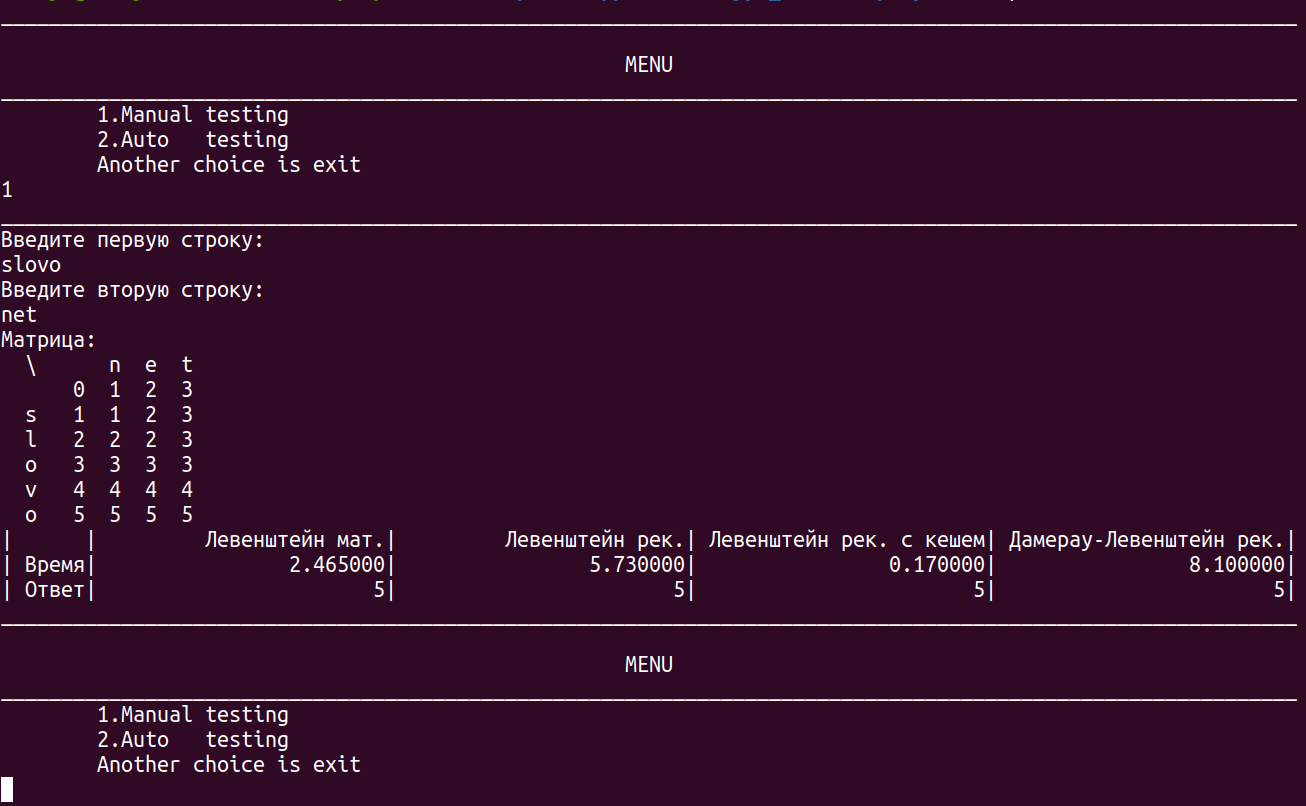
\includegraphics[scale=0.4]{workExample}}
    \caption{Ручное тестирование}
    \label{ris:work_example1}
  \end{figure}
  
\begin{figure}[H]
    \center{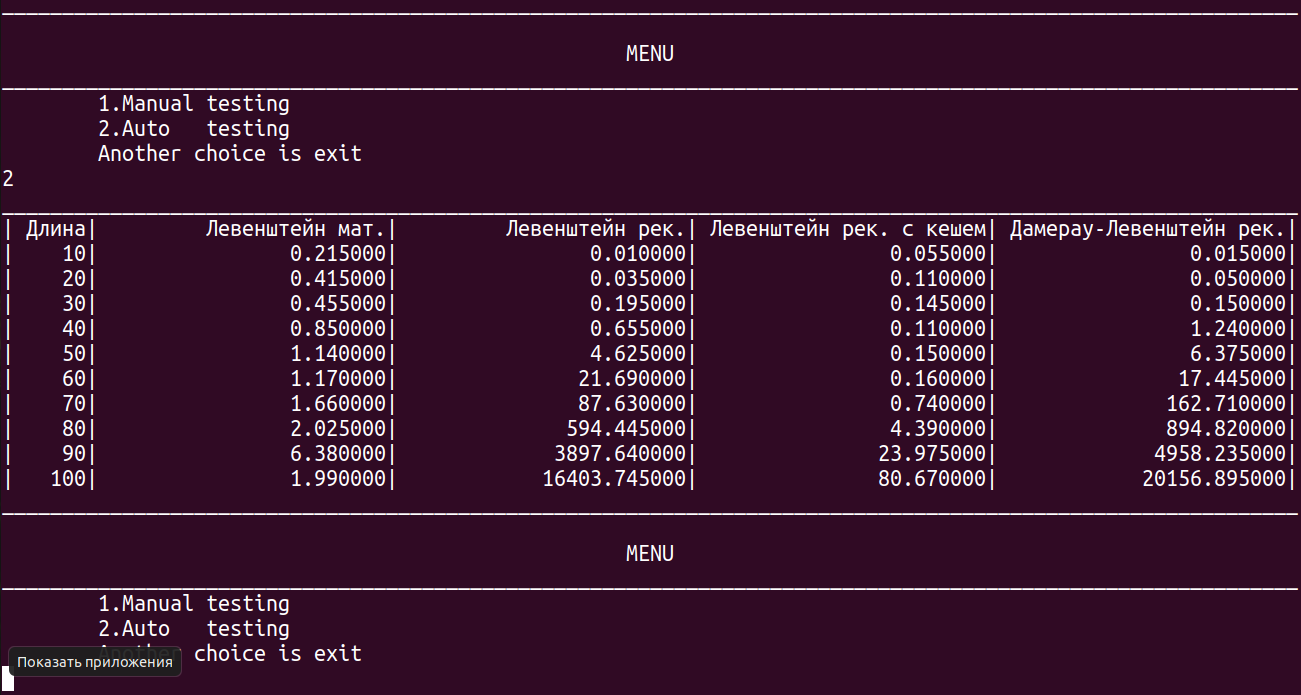
\includegraphics[scale=0.4]{workExample2}}
    \caption{Автоматическое тестирование}
    \label{ris:work_example2}
  \end{figure}

\section{Замеры времени}\label{experimentgraph}

На рисунках \ref{ris:graph1} и \ref{ris:graph2} показаны графические результаты сравнения исследуемых алгоритмов по времени. 

\begin{figure}[H]
    \center{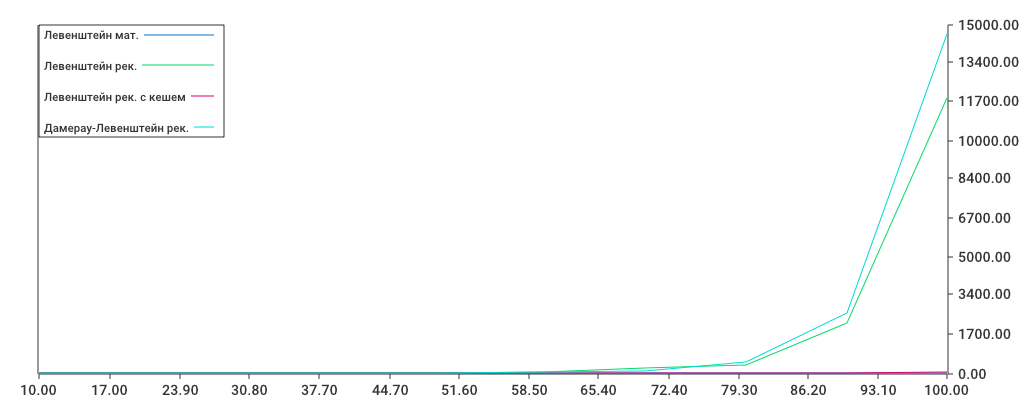
\includegraphics[scale=0.4]{../Lab1/output.png}}
    \caption{Сравнение всех 4 исследуемых алгоритмов по времени}
    \label{ris:graph1}
\end{figure}

\begin{figure}[H]
    \center{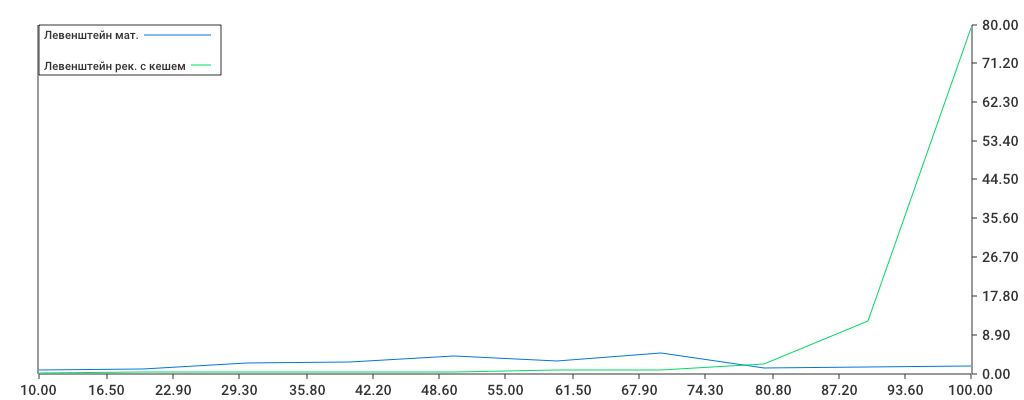
\includegraphics[scale=0.4]{../Lab1/output2.png}}
    \caption{Сравнение матричного и рекурсивного с кешем алгоритмов поиска расстояния Левенштейна}
    \label{ris:graph2}
\end{figure}


\section{Вывод экспериментальной части}\label{experimentresult}

Таким образом, по графикам подтвердилось предположение, что самый эффективный алгоритм поиска расстояния Левенштейна
из рассматриваемых в работе – рекурсивный метод с кешем. Рекурсивный алгоритм поиска расстояния Дамерау - Левенштейна дольше, чем 
рекурсивный алгоритм Левенштейна, что объясняется дополнительными операциями поиска перепутанных букв: (fd -> df).




\chapter{Заключение}\label{exit}

В данной работе был проведен обзор алгоритмов поиска расстояния Левенштейна и Дамерау-Левенштейна. 
Изучены алгоритмы поиска расстояния между строками: рекурсивные алгоритмы поиска расстояния Левенштейна 
и Дамерау-Левенштейна, рекурсивный алгоритм с кешем поиска расстояния Левенштейна, матричный алгоритм поиска Левенштейна. 
Получены практические навыки реализации исследуемых алгоритмов на языке программирования Go. 
Проведён сравнительный анализ алгоритмов по затрачиваемым ресурсам (зависимость времени от длины массива). 
Экспериментально подтверждены различия в эффективности алгоритмов с указанием лучших и худших случаев. 
При сравнении данных алгоритмов получены следующие результаты: самый эффективный алгоритм поиска расстояния Левенштейна 
из рассматриваемых в работе - рекурсивный алгоритм с кешем.




%\chapter*{Список литературы}\label{Bibliography}
\addcontentsline{toc}{chapter}{Список литературы}
\renewcommand\bibname{Список литературы}
\bibliographystyle{utf8gost705u}  % стилевой файл для оформления по ГОСТу
\nocite{*}
\bibliography{5.PartBiblio}          % имя библиографической базы (bib-файла)

%\printbibliography

\end{document}
